\let\negmedspace\undefined
\let\negthickspace\undefined
\documentclass[article]{IEEEtran}
\usepackage[a5paper, margin=10mm, onecolumn]{geometry}
%\usepackage{lmodern} % Ensure lmodern is loaded for pdflatex
\usepackage{tfrupee} % Include tfrupee package

\setlength{\headheight}{1cm} % Set the height of the header box
\setlength{\headsep}{0mm}     % Set the distance between the header box and the top of the text

\usepackage{gvv-book}
\usepackage{gvv}
\usepackage{cite}
\usepackage{amsmath,amssymb,amsfonts,amsthm}
\usepackage{algorithmic}
\usepackage{graphicx}
\usepackage{textcomp}
\usepackage{xcolor}
\usepackage{txfonts}
\usepackage{listings}
\usepackage{enumitem}
\usepackage{mathtools}
\usepackage{gensymb}
\usepackage{comment}
\usepackage[breaklinks=true]{hyperref}
\usepackage{tkz-euclide} 
\usepackage{listings}                                       
\def\inputGnumericTable{}                                 
\usepackage[latin1]{inputenc}                                
\usepackage{color}                                            
\usepackage{array}                                            
\usepackage{longtable}                                       
\usepackage{calc}                                             
\usepackage{multirow}                                         
\usepackage{hhline}                                           
\usepackage{ifthen}                                           
\usepackage{lscape}

\renewcommand{\thefigure}{\theenumi}
\renewcommand{\thetable}{\theenumi}
\setlength{\intextsep}{10pt} % Space between text and floats

\numberwithin{figure}{enumi}
\renewcommand{\thetable}{\theenumi}

% Marks the beginning of the document
\begin{document}
\bibliographystyle{IEEEtran}
\title{NCERT-6.5.24}
\author{EE24BTECH11039 - MANDALA RANJITH}
{\let\newpage\relax\maketitle}

\section*{Proof Using Gradient Descent}
\noindent\textbf{Question: }  
Show that the right circular cone of least curved surface and given volume has an altitude equal to $\sqrt{2}$ time the radius of the base.\\ \\
\noindent\textbf{Solution: } 



\subsection*{Objective Function and Constraint}

The \textbf{Curved Surface Area (CSA)} of the cone is:
\begin{align}
\text{CSA} &= \pi r \sqrt{r^2 + h^2}.
\end{align}

The volume constraint is:
\begin{align}
V &= \frac{1}{3} \pi r^2 h,
\end{align}
which gives:
\begin{align}
h &= \frac{3V}{\pi r^2}.
\end{align}

Substituting \(h\) into the CSA:
\begin{align}
\text{CSA}(r) &= \pi r \sqrt{r^2 + \left(\frac{3V}{\pi r^2}\right)^2}.
\end{align}

\subsection*{Gradient of CSA}

To minimize CSA, we compute its gradient:
\begin{align}
\frac{d}{dr}[\text{CSA}(r)] &= \pi \left(\sqrt{f(r)} + \frac{r}{2\sqrt{f(r)}} \cdot f'(r)\right),
\end{align}
where:
\begin{align}
f(r) &= r^2 + \left(\frac{3V}{\pi r^2}\right)^2, \\
f'(r) &= 2r - 2\left(\frac{3V}{\pi r^2}\right) \cdot \frac{6V}{\pi r^3}.
\end{align}

\subsection*{Gradient Descent Algorithm}

We minimize CSA using gradient descent:
\begin{align}
r_{\text{new}} &= r_{\text{old}} - \eta \frac{d}{dr}[\text{CSA}(r)],
\end{align}
where \(\eta\) is the learning rate.

\subsection*{Numerical Results}

After running gradient descent with:
\begin{itemize}
    \item Learning rate (\(\eta\)) = 0.01,
    \item Tolerance = \(10^{-6}\),
    \item Maximum iterations = 10,000,
\end{itemize}
we obtained:
\begin{align}
r &\approx 0.877308077654739, \\
h &\approx 1.2407009817987995, \\
\frac{h}{r} &\approx \sqrt{2}.
\end{align}


    \item \textbf{Computational Solution:}
    We use the method of gradient descent to find the minimum/maximum of the given function, since the objective function is convex. Since the coefficient of $r^2 > 0$, we expect to find a local minimum.
   \begin{align}
    r_{n+1} &= r_n - \alpha f'(r_n) \\
    r_{n+1} &= r_n - \alpha \left( 2r_n - 2 \frac{3V}{\pi r_n^2} \cdot \frac{6V}{\pi r_n^3} \right) \\
    r_{n+1} &= r_n - 2\alpha r_n - 2\alpha \frac{3V}{\pi r_n^2} \cdot \frac{6V}{\pi r_n^3}.
\end{align}

    \subsection*{Conclusion}

The gradient descent results confirm that the cone of least curved surface area for a given volume satisfies:
\begin{align}
h &= \sqrt{2}r.
\end{align}
\textbf{Alternate Computational Solution: }\newline

We can also solve it using $cvxpy$ module in python. On running the code we get,\newline
Minimum value of $h/r$ is, $1.4142135623730943cm$
, Optimal CSA is, $ 4.1880779495579015 cm^2$ \\\\
 Constraints are : $r>0$ and $h>0$ 


\begin{figure}[h!]
   \centering
   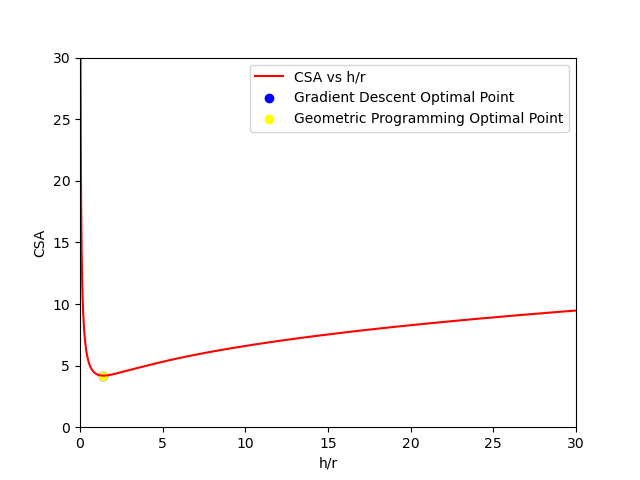
\includegraphics[width=\columnwidth]{figures/fig.png}
   \caption{$\frac{h}{r}$ vs $CSA$ graph and minimum point}
   \label{stemplot}
\end{figure}

\end{document}


